\section{Kapcsolási rajz}

\subsection{ESP8266}

\begin{table}[ht]
	\footnotesize
	\centering
	\begin{tabular}{ | c | c | c | c | c |}
		\toprule
		GPIO15 & GPIO0 & GPIO2 & mód & leírás \\
		\midrule
        Alacsony & Alacsony & Alacsony & UART & Kód letöltése UART-ról \\
        \hline
        Alacsony & Magas & Magas & Flash & Boot SPI Flash-ből \\
        \hline
		Magas & x  & x & SDIO & Boot SD kártyáról \\
		\bottomrule
	\end{tabular}
	\caption{ESP8266 boot módok}
	\label{tab:TabularExample}
\end{table}
% alap lábbekötések
% A modul programozása egy 6 pines csatlakozón (Rx,Tx,RTS,DTS,5V,GND) keresztül UART segítségével történik.

\subsection{FET meghajtó áramkörök}
A mikrokontroller kimenetei lábai maximálisan 12 mA-al terhelhetőek, ezért szükséges különböző meghajtó áramkörök használatára. A modulon helyett kapott 2 db P-csatornás, illetve 6 db N-csatornás MOSFET meghajtó. Lehetőség van kiválasztani az egységeknél a kapcsolt feszültséget. Ez lehet 5v, illetve a bemeneti tápfeszültség, ami maximálisan 12v. Tovább külön beállítható az N-csatornás MOSFET-eknél fel/lehúzó ellenállásokkal, hogy mi legyen az alapértelmezett állapota.
\begin{figure}[!h]
    \centering
    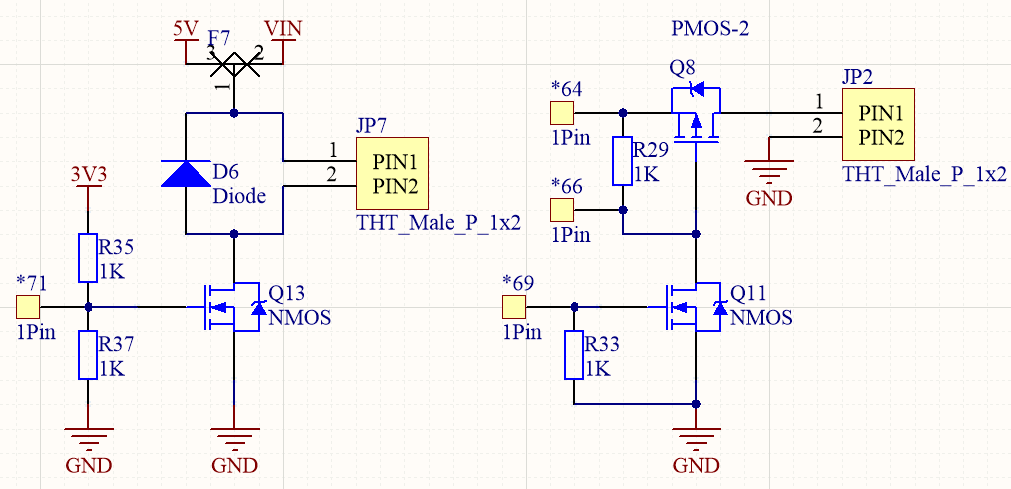
\includegraphics[width=150mm, keepaspectratio]{figures/n_p_driver.png}
    \caption{N és P csatornás MOSFET meghajtók}
    \label{fig:TeXstudio}
\end{figure}

\subsection{Optokapu}
2 db optokapunak lett hely kialakítva a panelon, amik például P-csatornás MOSFET meghajtóval kombinálva izolált vezérlést tesz lehetőve.


\subsection{Shift regiszterek}
A mikrokontrollernek mivel viszonylag kevés szabad GPIO lába áll rendelkezésre, ezért lehetőség van a különböző shift regiszterek használatával növelni az elérhető bemenetek és kimenetek számát, ha az alkalmazáshoz szükséges. A panelon 2db 8 bit-es SPI interfészel, illetve egy 16 bit-es I2C-vel rendelkező shift regiszter helyezhető el. A 8 bitesek egyike párhuzamos bemeneteket alakít sorossá. A másik pedig soros bemenetet alakít át párhuzamos kimenetekké. 
\begin{figure}[!h]
    \centering
    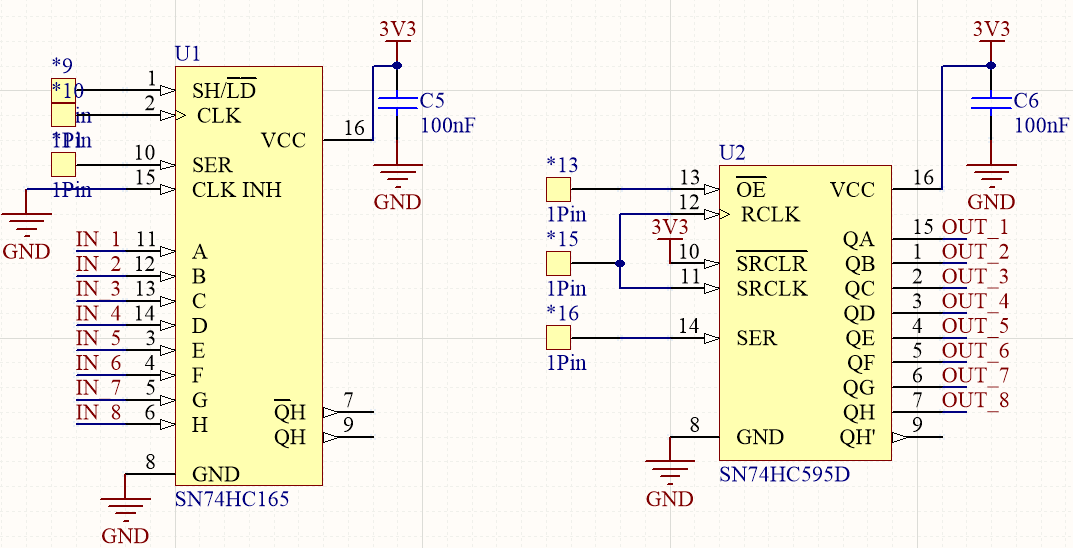
\includegraphics[width=150mm, keepaspectratio]{figures/8bit_shift_registers.png}
    \caption{8bites shift regiszterek kapcsolási rajza}
    \label{fig:TeXstudio}
\end{figure}
A 16 bites shift regiszteren külön konfigurálható, hogy milyen állapotban legyenek a lábai. Egy plusz funkció, hogy interrupt rendelhető bármelyik bemeneti módban lévő lábhoz. A felhasznált terület csökkentése érdekében, illetve mivel nem minden alkalmazáshoz szükséges plusz bemenet vagy kimenet, ezért a 16bites és a 8bites IC-k ki és bemenetei ugyanazokra a lábakra vannak kivezetve.
\begin{figure}[!h]
    \centering
    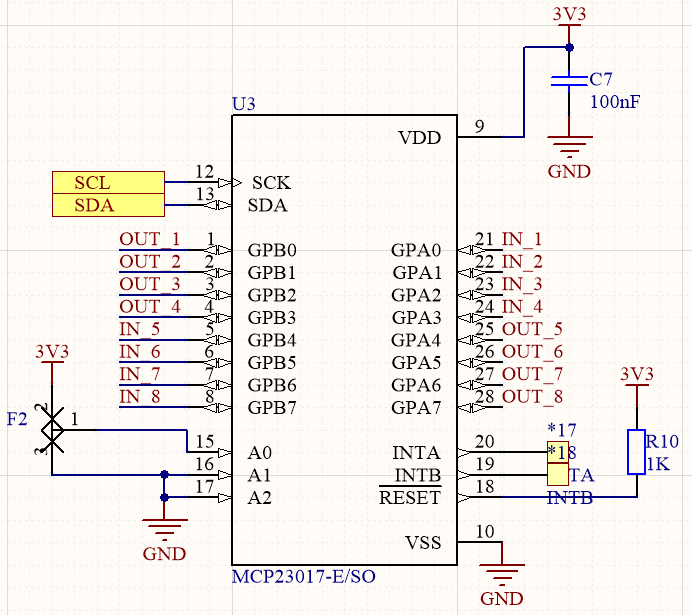
\includegraphics[width=100mm, keepaspectratio]{figures/16bit_shift_register.png}
    \caption{16bites shift regiszter kapcsolási rajza}
    \label{fig:TeXstudio}
\end{figure}



\subsection{I2C}
Az ESP8266-nak alapértelmezetten egy I2C interfésze van, ami szoftveresen van megvalósítva. Erre az interfészre kapcsolódik a panelon elhelyezkedő kijelző, hőmérséklet szenzor, illetve shift regiszter. Lehetőség van ezenkívűl további perifériák egyszerű csatlakoztatására is, mivel helyet kapott külön kivezetés tüskesorra is.

A panelon elhelyezett hőmérséklet szenzor egy LM75-ös digitális hőmérő, aminek SOP8 tokozása van. Számos más hőmérséklet, illetve párataratalom mérő szenzor is használható a megegyező lábkiosztásnak köszönhetően.
\begin{figure}[!ht]
    \centering
    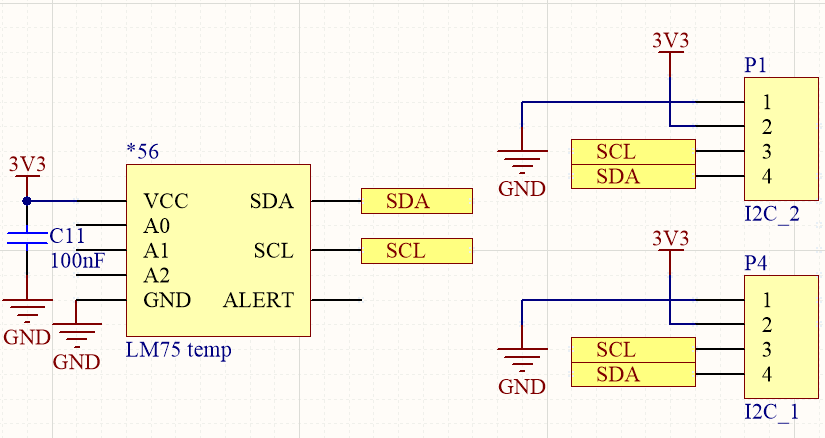
\includegraphics[width=130mm, keepaspectratio]{figures/i2c_devices.png}
    \caption{Hőmérséklet szenzor, illetve I2C kivezetések}
    \label{fig:TeXstudio}
\end{figure}

\subsection{Enkóder}
Lehetőség van egy kapcsolóval egybeépített enkóder bekötésére a panelon. Ennek a fő szerepe a kijelző által biztosított menürendszerben való navigálás. A kijelző hiánya esetében is több funkció rendelhető hozzá például a különböző kimenetek szabályzása. A beépített nyomógomb és egy interrupt segítségével például beállítható, hogy visszakapcsoljon alvás üzemmódból a mikrokontroller.

\subsection{Kijelzők, LED-ek}
\subsection{Tápellátás}